\documentclass[../main.tex]{subfiles}

\begin{document}
\section{Densities from Densities}


\begin{figure}
  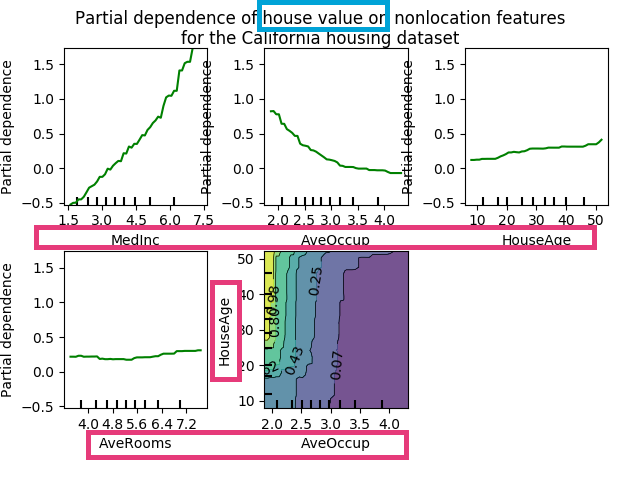
\includegraphics{partial_dependence}
  \caption{Taken from Scikit Learn\cite{_partial_????}, the line plots show how California housing prices are partially dependent on each x variable. The heat map illustrates the joint effect of the age the house and the number of occupants in the house.}
  \label{fig:partialdependence}
\end{figure}


One of the most straightforward ways to show dependencies is to plot one
variable against another, but those methods often exclude the effects of the
other variables in the datasets. Regression methods can be used to analyze the
ways in which one variable is partially dependent on many other variables in
the dataset\cite{_elements_2009}. As shown in figure~\ref{fig:partialdependence}, one way partial dependence line plots and two way partial dependence heat maps show how California housing prices are marginally dependent on each variable. 

While bar graphs and histograms can give a sense of the variability in
data, they are limited to showing the dispersion of the data only in how the measurements are spread out. This is somewhat limiting for very large datasets, so the box plot has evolved as a way to display more characteristics of the distribution \cite{wickham_40_2011}. While a simple box plot does not inherently show conditional dependencies, many derivations do. 

\begin{figure}
  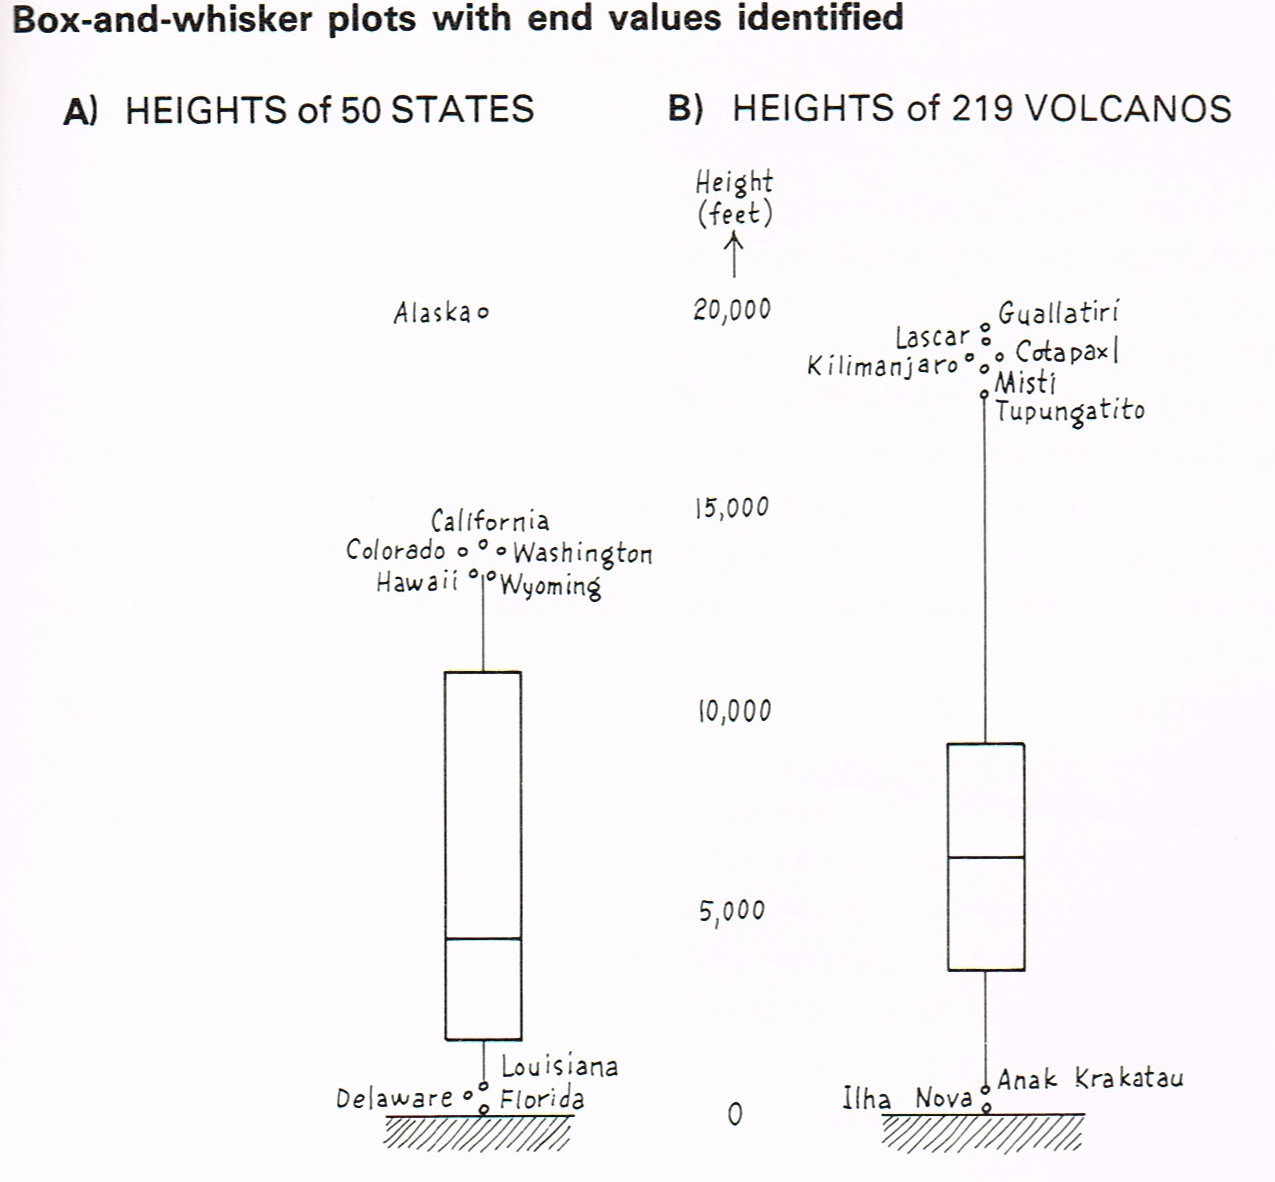
\includegraphics{boxplot}
  \caption{Tukey's 1977 example of the box plot from
    Exploratory Data Analytics\cite{tukey_exploratory_1977} illustrates how the box plot shows the distribution of topology of states and
    the distribution of volcanoes. The strength of the box and whisker is that the
    reader can quickly compare the two distributions and learn, for example,
    that volcanoes tend to span a shorter range of average heights, but that the
    extremes are much further from the center. Essentially, the distributions act as references for the other displayed distributions.}
  \label{fig:boxplot}
\end{figure}

Tukey's introduction to the box-plot \cite{tukey_exploratory_1977}, shown in
Figure~\ref{fig:boxplot} illustrates how the distributions of these 1 dimensional densities differ by category. While this graph shows the median, range between upper and lower interquartile, and lower and upper extreme, many authors have exploited the structure to convey more information about the data. Authors used different quantile levels \cite{hyndman_sample_1996}s or measures of outliers
\cite{frigge_implementations_1989, schwertman_identifying_2007}, or otherwise incorporated skewness, kurtosis, and other descriptive distributional statistics \cite{kim_more_2004, marmolejo-ramos_shifting_2015}.

While box plots were designed to visualize discrete observations, often there
are no discrete observations and instead the `observation` is a timeseries
curve (where the connections are as important as the individual points) or
spatial region. Understanding the distributions of functional observations
often relies first ordering the functions such that there's some measure of how close these functions are to each other--functional depth\cite{febrero_functional_2007},
bivariate score depth\cite{rob_j._hyndman_rainbow_2010}, and
bivariate kernel density estimation\cite{scott_multivariate_1992} are some examples. This
ordering then yields functional analogs to median and other percentile
metrics. For small values, the ordered curves can then be colored based on the
ordering metric \cite{rob_j._hyndman_rainbow_2010}, but this method is unwieldy for larger
ensembles.


\begin{figure}
  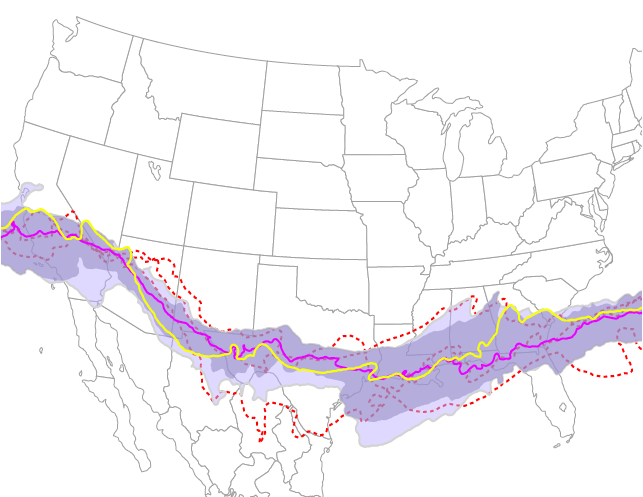
\includegraphics[width=.75\linewidth]{contour_weather}
  \caption{From \cite{whitaker_contour_2013}, the contour box plot method is used to show uncertainty in temperature ensembles while maintaining the temporal dimension of the data.}
  \label{fig:countour}
\end{figure}
Functional bag, box, and HDR plots \cite{rob_j._hyndman_rainbow_2010, sun_functional_2011} tend to be good at visualizing specific types of outliers, but are somewhat limited to only one functional distribution. A very common task is to compare ensembles, each a function of the same timeseries or geographic region. Contour box plots\cite{whitaker_contour_2013} aim to capture the variability of the
uncertainty via a band depth ordering metric. Each ensemble members band depth
is computed as sum of the probabilities that the observations in any given
ensemble fall within the max-min envelope defined by any two other
ensembles. The bands are then sorted by band depth such that the median is the
ensemble with about 50\% of its members whiten all envelopes formed by other
bands (so most centered). Outer bands are chosen according to the task at
hand, which in this paper is temperature visualizations. The authors argue that contour box plots are an improvement over spaghetti plots \cite{luo_visualizing_2003} because the spaghetti plots get nosy as the number of plots increase and so it's hard to tease out specific patterns. Instead in
Figure~\ref{fig:countour}, the authors remove most of the bands and instead visualize an outlying envelope(light gray) and a more central envelope(dark gray). It retains much of the information of
the spaghetti, but removes the visual noise of the lines.

One of the most common approaches for visualizing datasets that are structurally complex or have more than one or two levels of conditional dependencies is to built a toolkit comprising of many different basic visualization types. The calendar visualization described above is a simple example, and just like more complex tools it follows the design principal of overview-zoom/filter-details-on-demand \cite{shneiderman_eyes_1996} because these tools facilitate engagement with the data at the aggregate and encourage drilling down to the core. 
\end{document}


